\chapter{Auswirkungen}
\label{chapter:auswirkungen}

Wie bereits in \autoref{chapter:einleitung} gesagt, verwenden etwa 98\% aller Cyberangriffe eine Form des Social Engineerings.
Entsprechend sind viele Statistiken bezüglich grundsätzlicher Cyberkriminalität repräsentativ für Kriminalität im Bereich von Social Engineering und können äquivalent verwendet werden.

\section{Prävalenz}

Es existiert keine einheitliche Verteilung hinsichtlich Cyberangriffen auf globaler Ebene.
Stattdessen gibt es einen klar ersichtlichen Unterschied in der Quantität bezüglich derartiger Angriffe hinsichtlich der Länder, in denen das Angriffsziel liegt.
Die Kontinente Afrika und Asien weisen die geringsten Angriffszahlen auf; es werden also grundsätzlich Entwicklungsländer weniger häufig durch Cyberbedrohungen gefährdet.
Europa hat die größte Angriffsrate weltweit, wobei Russland explizit seit 2022 mit den meisten Angriffen um einen Faktor von 17 über dem Durchschnitt heraussticht \bcite{surfshark}.
Die nachfolgende Statistik stellt die Anzahl der Cyberangriffe in Deutschland repräsentativ für Industrieländer dar.

\begin{figure}[!htp]
    \centering
    \begin{tikzpicture}

        \draw (0cm,0cm) -- (11cm,0cm);  %Abzisse
        \draw (0cm,0cm) -- (0cm,-0.1cm);  %linkes Ende der Abzisse
        \draw (11cm,0cm) -- (11cm,-0.1cm) node [rotate=60, below, xshift=-0.4cm, yshift=0.2cm] {Jahr};  %rechtes Ende der Abzisse

        \draw (-0.1cm,0cm) -- (-0.1cm,5cm);  %Ordinate
        \draw (-0.1cm,0cm) -- (-0.2cm,0cm);  %unteres Ende der Ordinate
        \draw (-0.1cm,5cm) -- (-0.2cm,5cm) node [left] {Tsd.};  %oberes Ende der Ordinate

        \foreach \x [evaluate=\x as \i using int((\x + 0.0005) * 100 / 3)] in {0.3, 0.9,..., 4.8}  %Hilfslinien
            {
                \draw[gray!50, text=black] (-0.2cm,\x cm) -- (11cm,\x cm)
                node at (-0.5 cm,\x cm) {\small{\i}};
            };  %Beschriftung der Hilfslinien

        \foreach \i/\year [
            evaluate=\i as \y using (\i * 0.03),
            evaluate=\year as \x using ((\year-2007) * 0.6 + 0.5)
        ] in {
                34.2/2007,
                37.9/2008,
                50.3/2009,
                59.8/2010,
                59.5/2011,
                64.0/2012,
                64.4/2013,
                49.9/2014,
                45.8/2015,
                82.6/2016,
                86.0/2017,
                87.1/2018,
                100.5/2019,
                108.5/2020,
                124.1/2021,
                136.9/2022,
                134.4/2023
            }
            {
                \draw[fill=doc!60] (\x cm,0cm) rectangle (0.3cm+\x cm,\y cm) %die Säulen
                node at (0.2cm + \x cm,\y cm + 0.3cm) {\tiny{\i}}; %die Prozente über den Säulen
                \node[rotate=60, left] at (0.4cm +\x cm,-0.1cm) {\small{\year}}; %Säulenbeschriftung
            };

        \draw[red] (-0.1cm,0.7cm) -- (10.7cm,3.97cm); % fitting function: 6.062*(x)+23.3; 1 = year 2017 -> Tsd.


    \end{tikzpicture}
    \caption{Von der polizeilichen Kriminalstatistik (PKS) registrierte Straftaten im Bereich Cybercrime von den Jahren 2007 bis 2023. Zusammengetragene Werte aus den jährlich veröffentlichten Bundeslagebildern des Bundeskriminalamtes \bcite{pka}.
    Die in Rot dargestellte Trendkurve wurde anhand der ungerundeten Werte kalkuliert und weist einen linearen Korrelationskoeffizienten von 0.9304 auf.}
    % Linear correlation coefficient
    % 0.9304
    % Coefficient of determination
    % 0.8656
    % Average relative error, %
    % 13.7771 %
\end{figure}
\FloatBarrier

In der Statistik ist insgesamt ein klarer Aufwärtstrend zu erkennen. Bezüglich der Rezession in den Jahren 2014 und 2015 äußerte sich das Bundeskriminalamt wie folgt:
\qq{Das Gefährdungs- und Schädigungspotenzial durch Computerkriminalität bleibt unverändert hoch.} Es ist zu beachten, dass es sich lediglich um eine Rezession in der \qqq{Anzeigestatistik} handelt, welche die realen Zahlen nicht einwandfrei widerspiegelt \bcite{pka}.
Auf globaler Ebene lässt sich ebenfalls ein drastischer Anstieg seit der Coronapandemie 2019 feststellen, was zu zahlreichen expliziten Studien diesbezüglich führte. Beispielsweise veröffentlichte auch das BKA erstmalig eine Sonderauswertung (vergleiche \bcite{pka}).

Es ist zu beachten, dass bei Cybercrime von einem sehr großen Dunkelfeld auszugehen ist. 
\qq{Das heißt, dass vermutlich nur ein kleiner Teil der Straftaten in diesem Bereich zur Anzeige gebracht wird bzw. der Polizei und/oder den Strafverfolgungsbehörden bekannt ist.
Bereits 2013 hatte eine in Niedersachsen durchgeführte Dunkelfeldstudie ein Dunkelfeld von 91\% aller Cybercrimestraftaten errechnet.}\bcite{pka}

Demografisch findet in der Opferstatistik bezüglich Social Engineering ebenfalls ein Wandel statt.
Bis 2022 waren beständig Senioren im Alter von über 60 Jahren am stärksten von Cybercrime betroffen.
2022 waren erstmals seit 2015 Personen im Alter von 30 bis 39 die primären Opfer von Kriminalität im Internet.
Historisch ist zu erkennen, dass junge Menschen unter 20 Jahren am robustesten gegen derartige Gefährdungen sind, wobei diese in den letzten Jahren eine der höchsten Zuwächse (von 6\% jährlich) zu verzeichnen haben \bcite{surfshark}. 

Innerhalb der Angriffsvektoren von Social Engineering war Phishing seit Mitte der 1990er konsistent am verbreitetsten.
Dem Data Breach Investigation Report von Verizon aus dem Jahr 2022 zufolge sind etwa 70\% aller Social Engineering Angriffe dem Phishing zuzuordnen.
Pretexting liegt hier bei etwa 30\%\footnote{In der Summe ergeben sich in der Statistik von Verizon mehr als 100\%, da einzelne Angriffe gegebenenfalls mehrere Angriffsmethoden verwenden.}\bcite{verizon2022}.
Im Data Breach Investigation Report von Verizon 2024 hingegen hat Pretexting mit über 40\% die meiste Verwendung gefunden, wobei Phishing erstmalig nicht an prominentester Stelle mit circa 30\% auf Platz 2 sank \bcite{verizon2024}.
Der Grund hierfür ist, dass sich insbesondere der \qqq{Business E-Mail Compromise (BEC)} Angriff in den letzten Jahren durchsetzte und nach aktuellsten Zahlen (von Verizon) alleine mehr als 50\% der Vorfälle im Social Engineering Muster darstellt.
\qqq{BEC} als Angriffsvektor wird als Pretexting eingestuft, und macht Phishing somit große Konkurrenz. Da Pretexting selbst sich nicht durch technische, sondern soziale Kriteria (\autoref{sozial}) auszeichnet, ist es sinnvoll, sich mit der Psychologie hinter Social Engineering zu beschäftigen.

Ebenfalls einen starken Anstieg in der Verwendung hat \qqq{Extortion} (engl. \qqq{Erpressung}) zu verzeichnen.
Machte \qqq{Extortion} 2021 nur 2\% aller Social Engineering Angriffe aus, so war es 2023 bereits die dritt meist verwendete Angriffsmethode mit etwa 25\% insgesamt.
Neben Ransomware fällt auch beispielsweise \qqq{Sextortion} unter diesen Angriffsvektor, welche einen Großteil dieser Statistik ausmacht.
Gemeldete Fälle von \qqq{Sextortion} stiegen zwischen 2018 und 2022 um 88\% an \bcite{verizon2022,verizon2024,3_barracuda}.

Mögliche Gründe für den drastischen Anstieg in Cybercrime und damit Social Engineering sind wie folgt:

Laut dem globalen Report Digital 2021 hat sich die Gesamtzeit der Internetnutzung weltweit deutlich erhöht.
Der durchschnittliche Internetnutzer verbringt nun fast sieben Stunden täglich online und das über alle Endgeräte hinweg.
Im Vergleich zum Vorjahr ist hier ein Anstieg um 16 Minuten oder vier Prozent zu verzeichnen.
Januar 2022 gab es weltweit 4.66 Milliarden Internetnutzer, was ein Anstieg um 316 Millionen (7.3\%) im Vergleich zum Januar 2020 ist \bcite{digital}.
Es gibt also durchgängig mehr Menschen, welche das Internet täglich mehr nutzen.

Des Weiteren werden Social Engineering Angriffe immer simpler.
Vorgefertigte Werkzeuge wie das \qqq{Social-Engineer Toolkit (SET)} erlauben es schnell und einfach Social Engineering Angriffe durchzuführen.
Sie verfügen über zahlreiche Angriffsvektoren, welche öffentlich und frei zugänglich sind \bcite{set}.

Zuletzt scheint die Trendkurve der finanziellen Schäden drastischer zu steigen, also die Häufigkeit von Vorfällen.
Entsprechend richten individuelle Angriffe immer mehr finanziellen Schaden an.
Aus Sicht der Angreifer gilt somit also, dass Cyberkriminalität zunehmend lukrativer wird.

\section{Schaden}

Das finanzielle Motiv im Cybercrime ist nicht nur das primäre Motiv von Cyberkriminellen, sondern verdrängt alle anderen Motive nahezu vollständig.
Neben einer finanziellen Motivation existieren beispielsweise Spionage und persönliche Motive, wobei letztere statistisch außer Acht zu lassen sind.
Waren 2022 noch 11\% aller Data Breaches durch Spionage motiviert, so sind es 2023 gelegentlich 5\%.
Entsprechend stieg in diesen Jahren das finanzielle Motiv von 89\% auf 95\% an \bcite{verizon2022,verizon2024}.

Die folgende Abbildung bietet einen Überblick der durchschnittlichen Kosten eines Data Breaches. 

\begin{figure}[!htp]
    \centering
    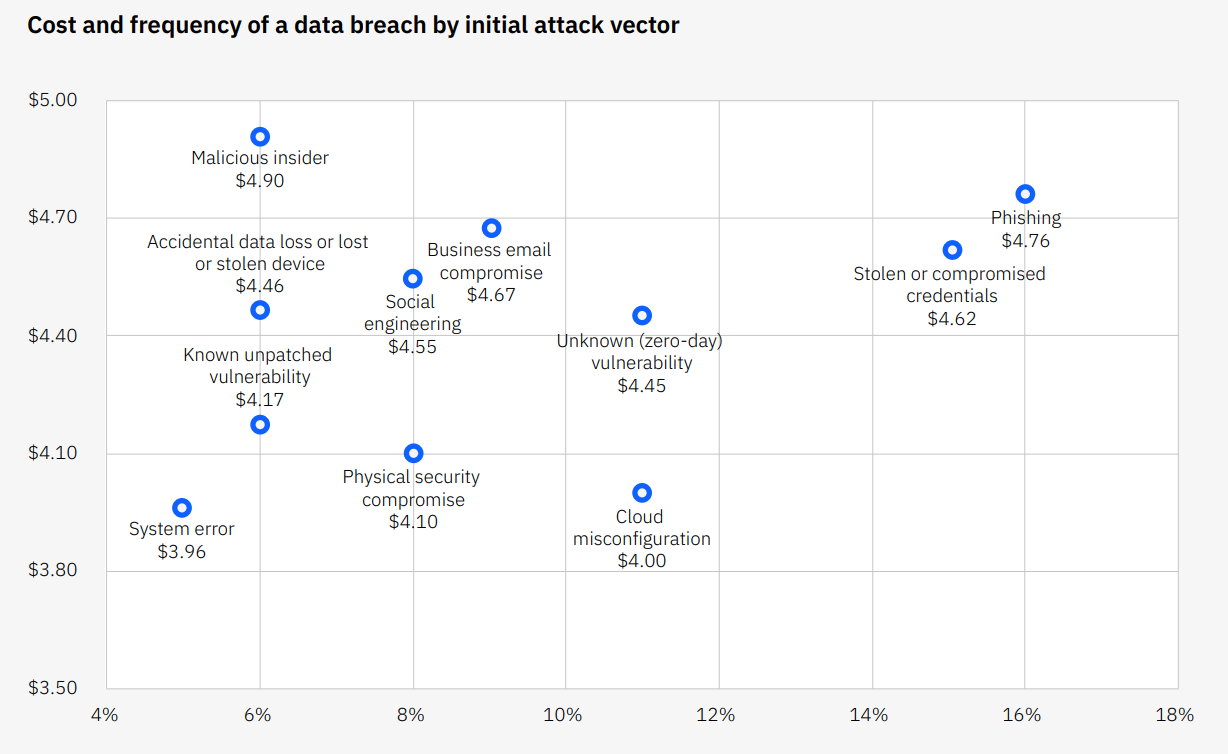
\includegraphics[width=\textwidth]{IBM_Data.Breach.Report.png}
    \caption{Die durchschnittlichen Kosten und Häufigkeiten von Data Breaches, geordnet nach ihrem initialen Angriffsvektor und gemessen in Millionen US-Dollar (2023)\bcite{6_ibmsecurity}.}
\end{figure}
\FloatBarrier

Der obigen Abbildung zufolge richtet ein Data Breach im Durchschnitt 4.45 Millionen US-Dollar an Schaden an, wobei Social Engineering als initialer Angriffsvektor mit 4.55 Millionen US-Dollar noch
über diesem Wert liegt \bcite{6_ibmsecurity}.
Es ist zu beachten, dass initiale Angriffsvektoren wie Phishing oder BEC ebenfalls unter Social Engineering verzeichnet werden könnten und damit den durchschnittlichen finanziellen Schaden weiter steigern würden. \\
Cybercrime hat 2015 einen globalen Schaden von 3 Billionen US-Dollar angerichtet, was sich bis 2021 auf 6 Billionen verdoppelt hat.
Bis 2025 wird prognostiziert, dass sich der weltweite Schaden auf etwa 10.5 Billionen US-Dollar beläuft \bcite{cyberventures}.

Der Verlust nach erfolgreichen Social Engineering Angriffen ist jedoch für Unternehmen weitreichender.
Neben dem direkten finanziellen Verlust durch den Diebstahl der Angreifer erleiden Unternehmen zusätzlich
Wiederherstellungskosten, da etwaige Daten verloren gegangen sind und Sicherheitslücken gefunden und repariert
werden müssen. Des Weiteren entsteht eine Betriebsdisruption, was zu indirektem finanziellen Schaden durch
Verlust von Produktivität führt. Zuletzt erleiden Unternehmen einen Reputationsschaden, was in vielen Fällen
den verheerendsten Faktor ausmacht, insbesondere für kleinere Firmen \bcite{agony}.
Zudem können Unternehmen rechtliche Konsequenzen haben, durch etwaige Haftungsklagen von Kunden oder Behörden, insofern Daten unausreichend gesichert waren.
Sollte der Angriff durch Industriespionage motiviert sein, erleiden Unternehmen zusätzlich einen Verlust von Wettbewerbsvorteilen beziehungsweise einen kompetitiven Schaden in der Marktwirtschaft, da zum Beispiel Geschäftsgeheimnisse gestohlen werden konnten \bcite{kotz}.

Individuen erleiden ebenfalls neben finanziellen- auch weitere Formen von Schäden.
Nicht außer Acht zu lassen ist der emotionale Schaden, da Personen oft in Folge einer erfolgreichen Manipulation als naiv dargestellt werden \bcite{10_bka}.
Reputationsschaden ist ebenfalls ein Faktor, der für Individuen beispielsweise bei Sextortion relevant ist.
\qq{Scham oder die Angst vor Reputationsverlust kann die Anzeigebereitschaft hemmen}\bcite{10_bka}, weshalb ein Social Engineering Angriff eine hohe durchschnittliche Zeit hat, um überhaupt identifiziert zu werden (MTTI\footnote{Mean Time to Identify}).
Der MTTI von Social Engineering liegt bei 218 Tagen, insofern er überhaupt entdeckt wird. Zusammen mit der durchschnittlichen Zeit von etwa 80 Tagen einen Angriff einzudämmen (MTTC\footnote{Mean Time to Contain}), vergehen ungefähr 300 Tage, bis ein Data Breach behoben wird \bcite{6_ibmsecurity}.
